\chapter{The O'Briens in Ireland}

The family of William O'Brien\index{O'Brien!William\textsuperscript{1}} and Mary Sexton\index{Sexton!Mary\textsuperscript{1}}\index{O'Brien!Mary\textsuperscript{1} (Sexton)} came to America from the town of Watergrasshill\index{Ireland!Watergrasshill, County Cork} in County Cork, Ireland.\index{Ireland!County Cork}\cite{Edward2OBrienNaturalization:1,Michael2OBrienNaturalization:1,Margaret3DooleyBaptism:1} The village of Watergrasshill\index{Ireland!Watergrasshill, County Cork} is situated mostly within the civil parish of Ardnageehy\index{Ireland!Ardnageehy, County Cork|see{Watergrasshill, County Cork}} and partly within Kilquane,\index{Ireland!Kilquane, County Cork} in the larger barony of Barrymore,\index{Ireland!Barrymore (Barony), County Cork} on the main road between Cork\index{Ireland!Cork (city)} and Dublin.\index{Ireland!Dublin}\cite{TopographicalDictionary} The name Watergrasshill\index{Ireland!Watergrasshill, County Cork} was originally ``Watercress Hill,'' and in Irish is \textit{Cnoc\'{a}n-na-biolraighe} (Knockaun-na-billery).\cite{LocalNames}

\begin{figure}
	\centering
	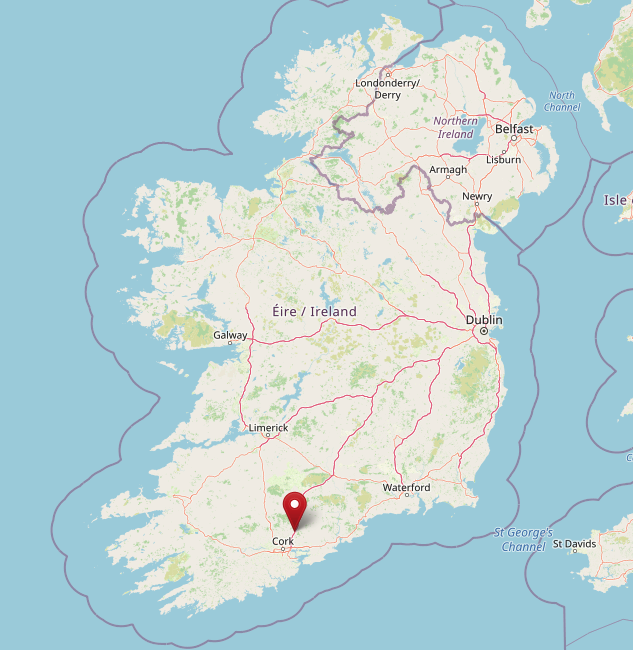
\includegraphics[width=\textwidth]{ireland}
	\caption{Map of Ireland with pin indicating the location of Watergrasshill\index{Ireland!Watergrasshill, County Cork}.}
	\label{fig:IrelandMap}
\end{figure}

\begin{figure}
	\centering
	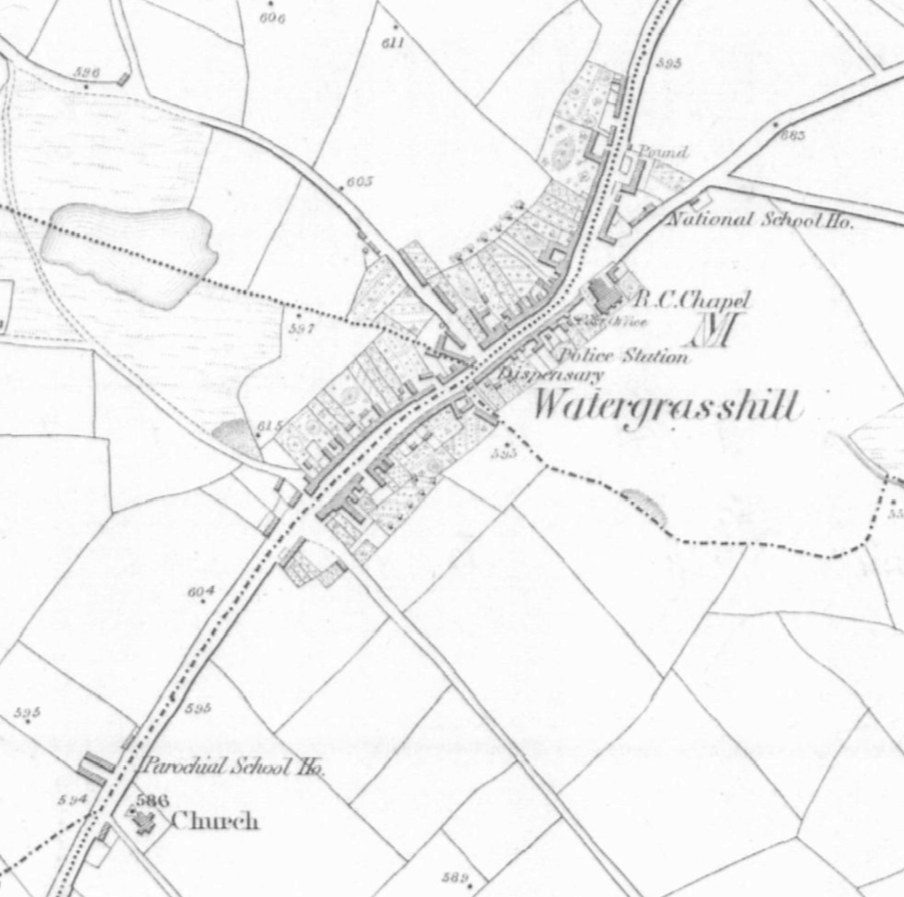
\includegraphics[width=\textwidth]{watergrasshill_cropped}
	\caption{Historic map of Watergrasshill (1829--1841)\index{Ireland!Watergrasshill, County Cork}}
	\label{fig:WatergrasshillMap}
\end{figure}

Watergrasshill\index{Ireland!Watergrasshill, County Cork} was a small town of 801 inhabitants in 1841, when William\index{O'Brien!William\textsuperscript{1}} and his family lived there prior to their emigration to the U.S. By 1871 the population had dropped to 143.\cite{Population} Some of this population loss was likely due to the famine,\index{famine} but the arrival of the railroad\index{railroad} may also have played a role. The Great Southern and Western Railway\index{Great Southern and Western Railway, The}\index{railroad} reached the City of Cork\index{Ireland!Cork (city)} in 1849.\cite{Bianconi:1} Two people performing land valuations included their impressions of Watergrasshill\index{Ireland!Watergrasshill, County Cork} and its transformation. D.\ Quinn\index{Quinn!D.\} wrote in Feb 1849:

\begin{quote}
	This Town is Poor, but a great deal is done in the way of ``Carmen's Stages,'' it being on the Dublin\index{Ireland!Dublin} line to Cork\index{Ireland!Cork (city)} and half way (11 miles) from the latter City to Fermoy\index{Ireland!Fermoy, County Cork} -- a good deal of benefit is done the Town by these persons ---\cite{HouseIntro:1}
\end{quote}

J.\ Montgomery\index{Montgomery!J.\} wrote in Dec 1852 and sometime prior:

\begin{quote}
	2 coaches \& Bianconis\footnote{Charles Bianconi\index{Bianconi!Charles} was an Italian entrepreneur who operated passenger coaches between cities throughout Ireland.\cite{Bianconi:2}} can pass through the village daily \& change Horses here -- one or two individuals are thus making pretty well by this -- by the rent for stabling \&c -- \& when the railway to Cork\index{Ireland!Cork (city)}\index{railroad} is finished, it will lose a good part of this advantage ---
	
	It has lost a great deal of it now -- (1852) but it is the best of the little villages in this neighborhood although poor enough -- Poor Rates are low -- only 1/7th for 1832 \& none at all in 1837 -- Those made a moderate val\textsuperscript{n}.\ considering these circumstances.\cite{HouseIntro:2}
\end{quote}

There are few Irish records available covering the early 19th century. Civil registration of births, marriages, and deaths didn't fully occur in Ireland\index{Ireland} until 1864.\cite{Grenham:1} Census records\index{Ireland!Census}\index{Census!Ireland} prior to 1901 were mostly lost in a 1922 fire at the Public Records Office.\cite{Grenham:18} However, there are O'Briens in Watergrasshill\index{Ireland!Watergrasshill, County Cork} who appear in name directories and Griffith's Valuation\index{Griffith's Valuation} records from the time period when William's\index{O'Brien!William\textsuperscript{1}} family lived in the area. It's possible that these sources may reveal some small details about the family's life in Ireland.\index{Ireland}
\begin{comment}
[ADD PARISH REGISTER AVAILABLE DATES AND MARGARET DOOLEY BAPTISM]
Watergrasshill and Glenville Parish
Parish records exist for the following: Baptisms From 1836
Marriages From 1864
Confirmations From 1955
https://wghparish.ie/about/
Watergrasshill; County of Cork; Diocese of Cork and Ross. Baptisms, Nov. 1840 to Jan. 1841, p. 27. http://registers.nli.ie/registers/vtls000635355#page/27
Image: Margaret_Dooley_baptism
27 Dec 1840
\end{comment}

There is a ``W\textsuperscript{m}.\ Brien'' listed in the town of Watergrasshill\index{Ireland!Watergrasshill, County Cork} who was leasing a house with a yard and garden.\cite{Valuation1849:1} The Feb 1849 revision has William's name crossed out and the word ``Vact.''\ written, indicating that the house was vacant and William had moved away.\cite{House1849} See William O'Brien's profile for more details about the available records.

There are no other William O'Briens or similar name variants listed in Watergrasshill,\index{Ireland!Watergrasshill, County Cork} although other O'Briens in town include Denis,\index{O'Brien!Denis}\cite{Valuation1849:2} Owen,\index{O'Brien!Owen}\cite{Valuation1849:3} Patrick,\index{O'Brien!Patrick}\cite{Valuation1849:4} and Margaret.\index{O'Brien!Margaret}\cite{Valuation1849:5}

The final version of Griffith's Valuation,\index{Griffith's Valuation} published in 1853, shows only Owen O'Brien\index{O'Brien!Owen}\cite{Griffiths:46,Griffiths:90:1} and Patrick O'Brien\index{O'Brien!Patrick}\cite{Griffiths:90:2} remaining in Watergrasshill.\index{Ireland!Watergrasshill, County Cork}\footnote{There are two properties occupied by an Owen O'Brien\index{O'Brien!Owen} and two properties occupied by a Patrick O'Brien.\index{O'Brien!Patrick} It's unknown whether these are four separate individuals or if there may be multiple properties rented by the same individuals.} By 1901 it appears that all O'Briens had left Watergrasshill,\index{Ireland!Watergrasshill, County Cork} as none are listed in the 1901 or 1911 census.\index{Ireland!Census}\index{Census!Ireland}\cite{1901IrishCensus,1911IrishCensus}

The departure of the O'Brien family\index{O'Brien!family} from Ireland\index{Ireland} corresponded with the ending years of the Irish potato famine,\index{famine} also known as the Great Famine, which lasted from 1845--1849. During this time, there were between 1.5 and 3 million famine-related deaths in Ireland and 1 million people left Ireland for North America.\cite{Smith:469}

\begin{figure}
	\centering
	\includegraphics[width=\textwidth]{famine_relief_commission}
	\caption{Excerpt from the \textit{Constitution} newspaper}
	\label{fig:FamineRelief}
\end{figure}

Watergrasshill\index{Ireland!Watergrasshill, County Cork} was a poor town in the 1840s that was largely sustained by horse travel between Dublin\index{Ireland!Dublin} and Cork.\index{Ireland!Cork (city)} With the loss of that business to the railway\index{railroad} and the effects of the famine,\index{famine} it made sense for the O'Brien family\index{O'Brien!family} to look for new opportunities in America.

\begin{thebibliography}{999}
	\addcontentsline{toc}{section}{\bibname}

% Chapter 1: The O'Briens in Ireland

\bibitem{Edward2OBrienNaturalization:1}
Edward O Brien primary declaration of intention (1854), no.\ 487, 
District of Massachusetts; 
Record Group 21: Records of the District Courts of the United States; 
National Archives at Boston, Waltham, Massachusetts;
viewed at ``Massachusetts, State and Federal Naturalization Records, 1798--1950,''
database with images, \textit{Ancestry.com} (\url{https://www.ancestry.com/search/collections/2361/} : viewed on 23 Mar 2020), image 858.

\bibitem{Michael2OBrienNaturalization:1}
Michael OBrien petition for naturalization (1868), 
Massachusetts Superior Court, Suffolk County; 
Oct term 1868 (Letters L--Z), Film \# 007795438,
viewed at ``Primary and final declarations of intention and naturalizations, 1864--1888 and card index 1856--1884,''
database with images, \textit{FamilySearch} (\url{https://www.familysearch.org/ark:/61903/3:1:3Q9M-CS9H-83DG-G}) : viewed on 23 Mar 2020), image 1859.

\bibitem{Margaret3DooleyBaptism:1}
Watergrasshill \& Glenville Parish (Watergrasshill, Ireland), ``Historical Baptisms from 1836--1901,'' database, ``Margaret Dooly'' baptism, 27 Dec 1840; \textit{Watergrasshill \& Glenville Parish Archives.} \url{http://www.wghparish.ie/index.php/archives/baptisms-1836-1901/easytablerecord/1-baptisms/7008} : viewed on 17 Apr 2019.

\bibitem{TopographicalDictionary}
Samuel Lewis, \textit{A Topographical Dictionary of Ireland}, vol. 2 (London: S.\ Lewis \& Co.\, 1837), 695.

\bibitem{LocalNames}
Patrick Weston Joyce, \textit{Irish Local Names Explained} (Dublin: The Educational Co.\ of Ireland, Limited, 1922), 93.

\bibitem{Population}
\textit{Census of Ireland, 1871}, Part 1, Vol. 2 (Dublin: Alexander Thom, 1873), 140; viewed at \textit{Histpop - The Online Historical Population Reports Website} (\url{http://www.histpop.org/}) : viewed on 23 Mar 2020.

\bibitem{Bianconi:1}
Brian Igoe, ``Charles Bianconi and The Transport Revolution, 1800 -- 1875,'' blog post, published 14 Dec 2012; \textit{The Irish Story} (\url{https://www.theirishstory.com/2012/12/14/charles-bianconi-and-the-transport-revolution-1800-1875/} : viewed 27 Mar 2020).

\bibitem{HouseIntro:1}
``House Book, Town of Watergrasshill, County of Cork, Barony of Barrymore, Feby 1849,'' title page; viewed at ``Ireland, Valuation Office Books, 1831--1856,'' database with images, \textit{FamilySearch} (\url{https://www.familysearch.org/ark:/61903/3:1:3QS7-994N-YCXK} : viewed 27 Mar 2020), film \#007246869, image 433.

\bibitem{Bianconi:2}
Brian Igoe, ``Charles Bianconi and The Transport Revolution, 1800 -- 1875,'' blog post, published 14 Dec 2012; \textit{The Irish Story} (\url{https://www.theirishstory.com/2012/12/14/charles-bianconi-and-the-transport-revolution-1800-1875/} : viewed 27 Mar 2020).

\bibitem{HouseIntro:2}
``House Book, Town of Watergrasshill, County of Cork, Barony of Barrymore, Feby 1849,'' title page; viewed at ``Ireland, Valuation Office Books, 1831--1856,'' database with images, \textit{FamilySearch} (\url{https://www.familysearch.org/ark:/61903/3:1:3QS7-994N-YCXK} : viewed 27 Mar 2020), film \#007246869, image 433.

\bibitem{Grenham:1}
John Grenham, \textit{Tracing your Irish Ancestors} (Dublin: Gill Books, 2019), 1.

\bibitem{Grenham:18}
John Grenham, \textit{Tracing your Irish Ancestors} (Dublin: Gill Books, 2019), 18.

\bibitem{Valuation1849:1}
``Ireland, Valuation Office Books, 1831-1856,'' database with images, \textit{FamilySearch} (\url{https://familysearch.org/ark:/61903/3:1:3QS7-994N-TW7T} : viewed on 19 Sep 2020), Cork > Ardnageehey > Watergrasshill > image 4, citing ``Wm.\ Brien'' at lot 29-50.

\bibitem{House1849}
``House Book, Town of Watergrasshill, County of Cork, Barony of Barrymore, Feby 1849,'' Houses in Town of Watergrasshill, Parish of Ardnageehy, Townland of Tinageragh, No.\ 44 (original), Lot 29 (revised), Wm Brien; viewed at ``Ireland, Valuation Office Books, 1831--1856,'' database with images, \textit{FamilySearch} (\url{https://www.familysearch.org/ark:/61903/3:1:3QS7-994N-YC62} : viewed 26 Mar 2020), film \#007246869, image 442.

\bibitem{Valuation1849:2}
``Ireland, Valuation Office Books, 1831-1856,'' database with images, \textit{FamilySearch} (\url{https://familysearch.org/ark:/61903/3:1:3QS7-994N-TW7T} : viewed on 19 Sep 2020), Cork > Ardnageehey > Watergrasshill > image 6, citing ``Denis Brien'' at lot 11-18.

\bibitem{Valuation1849:3}
``Ireland, Valuation Office Books, 1831-1856,'' database with images, \textit{FamilySearch} (\url{https://familysearch.org/ark:/61903/3:1:3QS7-994N-TW7T} : viewed on 19 Sep 2020), Cork > Ardnageehey > Watergrasshill > image 6, citing ``Owen Brien'' at lot 26-5.

\bibitem{Valuation1849:4}
``Ireland, Valuation Office Books, 1831-1856,'' database with images, \textit{FamilySearch} (\url{https://familysearch.org/ark:/61903/3:1:3QS7-994N-TW7T}: viewed on 19 Sep 2020), Cork > Ardnageehey > Watergrasshill > image 7, citing ``Pk. Brien'' at lot 26-10.

\bibitem{Valuation1849:5}
``Ireland, Valuation Office Books, 1831-1856,'' database with images, \textit{FamilySearch} (\url{https://familysearch.org/ark:/61903/3:1:3QS7-994N-TW7T} : viewed on 19 Sep 2020), Cork > Ardnageehey > Watergrasshill > image 11, citing ``Margt Brien'' at lot 34-22.

\bibitem{Griffiths:46}
Richard Griffith, \textit{General Valuation of Rateable Property in Ireland}, County of Cork, Poor Law Union of Cork, Fermoy, and Middleton, Barony of Barrymore (Dublin: Alexander Thom, 1853), 46, citing Owen Brien at plot 23-3, Patrick Brien at plot 23-5, and Patrick Brien at plot 23-8.

\bibitem{Griffiths:90:1}
Richard Griffith, \textit{General Valuation of Rateable Property in Ireland}, County of Cork, Poor Law Union of Cork, Fermoy, and Middleton, Barony of Barrymore (Dublin: Alexander Thom, 1853), 90, citing Owen Brien at plot 26-17.

\bibitem{Griffiths:90:2}
Richard Griffith, \textit{General Valuation of Rateable Property in Ireland}, County of Cork, Poor Law Union of Cork, Fermoy, and Middleton, Barony of Barrymore (Dublin: Alexander Thom, 1853), 90, citing Owen Brien at plot 26-17.

\bibitem{1901IrishCensus}
The National Archives of Ireland, ``Census of Ireland 1901/1911 and Census fragments and substitutes, 1821-51,'' database, \url{http://www.census.nationalarchives.ie/}, Census Years > 1901 > Cork > Watergrasshill > Watergrasshill Town.

\bibitem{1911IrishCensus}
The National Archives of Ireland, ``Census of Ireland 1901/1911 and Census fragments and substitutes, 1821-51,'' database, \url{http://www.census.nationalarchives.ie/}, Census Years > 1911 > Cork > Watergrasshill > Watergrasshill Town, part of.

\bibitem{Smith:469}
Cynthia E. Smith, ``The Land-Tenure System in Ireland: A Fatal Regime,'' \textit{Marquette Law Review}, vol.\ 76 issue 2 p.\ 469 (Winter 1993) \url{http://scholarship.law.marquette.edu/mulr/vol76/iss2/6}

\end{thebibliography}